% 图 18.3 —— 由 `checks/emit_hand.py` 自动拼出（probe 精测 + prims2 图元分解）
%%
% ⚠ 这是**稿子不是成品**：跑 `checks/checkhand.py 18.3` 看指标 + 看叠合图。
%%
%% ⚠ 待核：
%   · 本图 probe 报出阴影族 1 个 —— **本脚本不生成阴影**（要照原书手写）；prims2 的 strokes 里可能含阴影线，核对时留意别画重
%   · 可疑字形 1 项（空心圈 ⊙ 常被认成字母 o）—— 见文件末
%%
\documentclass[12pt]{standalone}
\usepackage{fontspec}
\setsansfont{Arial}
\newfontfamily\mfallback{DejaVu Sans}
\usepackage{tikz}
\begin{document}
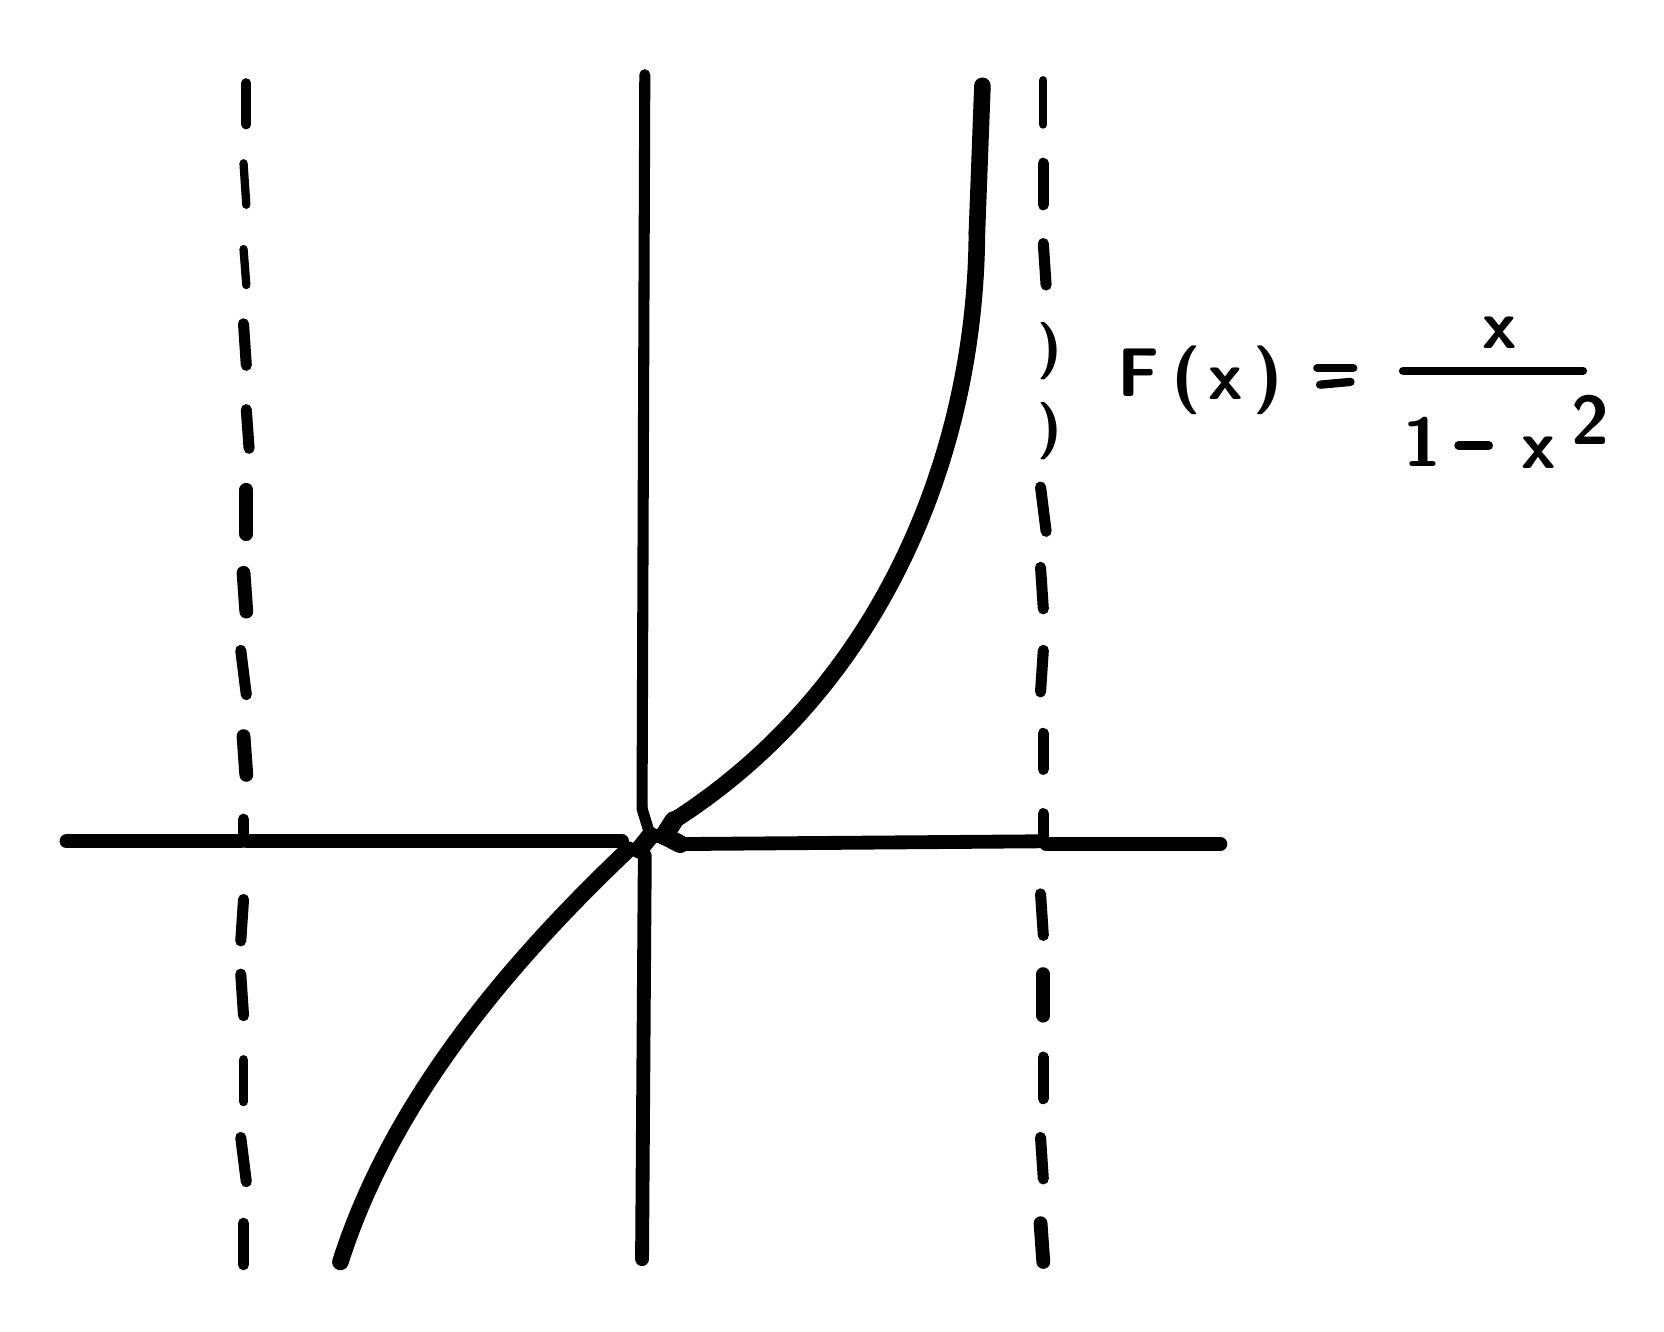
\begin{tikzpicture}[x=1pt, y=-1pt, line width=4.0pt, line cap=round, line join=round]

  %% ════ 直线段（prims2 的 strokes）════
  \draw[line width=4.0pt] (367.0,210.0) -- (366.0,195.0);
  \draw[line width=4.0pt] (78.0,315.0) -- (77.0,330.0);
  \draw[line width=3.0pt] (528.0,151.0) -- (517.0,151.0);
  \draw[line width=3.0pt] (466.0,123.0) -- (479.0,123.0);
  \draw[line width=5.0pt] (366.0,294.0) -- (235.8,295.0);
  \draw[line width=6.5pt] (235.8,295.0) -- (230.0,292.0);
  \draw[line width=4.0pt] (367.0,293.0) -- (367.0,284.0);
  \draw[line width=4.0pt] (77.0,401.0) -- (79.0,417.0);
  \draw[line width=4.0pt] (225.0,292.0) -- (222.0,282.2);
  \draw[line width=4.0pt] (222.0,282.2) -- (223.0,17.0);
  \draw[line width=5.0pt] (225.0,292.0) -- (230.0,292.0);
  \draw[line width=6.5pt] (225.0,292.0) -- (221.0,297.0);
  \draw[line width=4.0pt] (366.0,166.0) -- (368.0,182.0);
  \draw[line width=5.0pt] (366.0,432.0) -- (367.0,446.0);
  \draw[line width=3.0pt] (497.0,124.0) -- (562.0,124.0);
  \draw[line width=3.0pt] (79.0,93.0) -- (78.0,80.0);
  \draw[line width=5.0pt] (431.0,295.0) -- (368.0,295.0);
  \draw[line width=4.0pt] (367.0,416.0) -- (366.0,401.0);
  \draw[line width=5.0pt] (14.0,294.0) -- (77.0,294.0);
  \draw[line width=3.5pt] (79.0,20.0) -- (79.0,35.0);
  \draw[line width=5.0pt] (78.0,256.0) -- (79.0,270.0);
  \draw[line width=5.0pt] (222.0,445.0) -- (223.0,299.2);
  \draw[line width=3.0pt] (223.0,299.2) -- (221.0,297.0);
  \draw[line width=4.0pt] (78.0,432.0) -- (78.0,447.0);
  \draw[line width=3.0pt] (478.0,128.0) -- (467.0,129.0);
  \draw[line width=5.0pt] (79.0,167.0) -- (79.0,183.0);
  \draw[line width=4.0pt] (367.0,78.0) -- (368.0,93.0);
  \draw[line width=4.0pt] (77.0,342.0) -- (78.0,357.0);
  \draw[line width=6.0pt] (345.0,21.0) -- (343.0,74.3);
  \draw[line width=6.8pt] (233.5,286.5) -- (230.0,292.0);
  \draw[line width=4.0pt] (367.0,225.0) -- (366.0,240.0);
  \draw[line width=4.0pt] (78.0,286.0) -- (78.0,293.0);
  \draw[line width=5.0pt] (367.0,357.0) -- (367.0,342.0);
  \draw[line width=4.0pt] (77.0,225.0) -- (79.0,241.0);
  \draw[line width=3.0pt] (221.0,297.0) -- (218.0,297.0);
  \draw[line width=4.0pt] (78.0,107.0) -- (79.0,122.0);
  \draw[line width=5.0pt] (78.0,197.0) -- (79.0,211.0);
  \draw[line width=4.0pt] (367.0,268.0) -- (367.0,255.0);
  \draw[line width=3.5pt] (78.0,373.0) -- (78.0,388.0);
  \draw[line width=4.0pt] (366.0,313.0) -- (367.0,328.0);
  \draw[line width=3.0pt] (79.0,64.0) -- (78.0,49.0);
  \draw[line width=3.0pt] (367.0,19.0) -- (367.0,35.0);
  \draw[line width=4.0pt] (79.0,138.0) -- (80.0,152.0);
  \draw[line width=3.0pt] (217.0,296.0) -- (214.8,294.0);
  \draw[line width=5.0pt] (214.8,294.0) -- (79.0,294.0);
  \draw[line width=4.0pt] (367.0,49.0) -- (367.0,64.0);
  \draw[line width=4.0pt] (367.0,372.0) -- (367.0,387.0);

  %% ════ 曲线（prims2 的 curves —— 三段式，坐标同为 (y,x)）════
  \draw[line width=6.0pt] (343.0,74.3) .. controls (342.4,157.5) and (306.2,240.0) .. (233.5,286.5);
  \draw[line width=6.0pt] (113.0,446.0) .. controls (131.2,389.0) and (171.9,339.8) .. (217.0,297.0);

  %% ════ 标签（probe 直接给的 \node 行）════
  %% ⚠ 全部补了 fill=white：文字在最上层，否则与曲线交叉干扰
     \node[anchor=center,inner sep=0pt,fill=white,font=\fontsize{31.9}{39.9}\selectfont] at (532.1,110.1) {\textsf{\textbf{\textit{x}}}};   % box(522,99,18,18)
     \node[anchor=center,inner sep=0pt,fill=white,font=\fontsize{20.0}{25.0}\selectfont] at (369.5,116.8) {\textsf{\textbf{)}}};   % box(366,107,5,19)
     \node[anchor=center,inner sep=0pt,fill=white,font=\fontsize{30.6}{38.3}\selectfont] at (401.5,124.5) {\textsf{\textbf{\textit{F}}}};   % box(392,112,19,23)
     \node[anchor=center,inner sep=0pt,fill=white,font=\fontsize{30.7}{38.4}\selectfont] at (418.5,127.5) {\textsf{\textbf{(}}};   % box(414,113,8,28)
     \node[anchor=center,inner sep=0pt,fill=white,font=\fontsize{32.6}{40.7}\selectfont] at (448.1,127.5) {\textsf{\textbf{)}}};   % box(442,113,9,28)
     \node[anchor=center,inner sep=0pt,fill=white,font=\fontsize{31.0}{38.7}\selectfont] at (433.0,128.6) {\textsf{\textbf{\textit{x}}}};   % box(423,118,18,17)
     \node[anchor=center,inner sep=0pt,fill=white,font=\fontsize{24.7}{30.9}\selectfont] at (564.6,141.9) {\textsf{\textbf{2}}};   % box(558,133,12,17)
     \node[anchor=center,inner sep=0pt,fill=white,font=\fontsize{20.0}{25.0}\selectfont] at (369.5,145.8) {\textsf{\textbf{)}}};   % box(366,136,5,19)
     \node[anchor=center,inner sep=0pt,fill=white,font=\fontsize{28.9}{36.1}\selectfont] at (503.9,150.0) {\textsf{\textbf{1}}};   % box(496,139,9,21)
     \node[anchor=center,inner sep=0pt,fill=white,font=\fontsize{31.0}{38.7}\selectfont] at (546.0,153.6) {\textsf{\textbf{\textit{x}}}};   % box(536,143,18,17)

  % 钉死画布：否则超出的图元/控制点会把页面撑大，1:1 回比就失准
  \pgfresetboundingbox
  \path[use as bounding box] (0,0) rectangle (581,461);
\end{tikzpicture}
\end{document}

% ⚠ 待核清单（probe 拿不准，人眼过一遍）：
%   · 未识别/跳过：⑤ 跳过/未识别的字形
